\documentclass[a4paper, 14pt]{extarticle}

% Useful packages
\usepackage{amsmath, amsfonts, amssymb} % AMS math packages
\usepackage{graphicx} % For including graphics
\graphicspath{{figures/}}
\usepackage{siunitx} % For typesetting SI units
\usepackage[colorlinks=true, allcolors=black]{hyperref} % Hyperlinks with black color
\usepackage{grffile} % Improved file name support for graphics
\usepackage{subcaption} % Subfigure and subcaption support
\usepackage{float} % Improved float placement
\usepackage{setspace} % Set space between lines
\usepackage[11pt]{extsizes} % Extends document class options
\usepackage[numbers]{natbib} % For numeric citations

\usepackage{fancyhdr} % Customizing headers and footers
\setlength{\headheight}{0pt} % Setting the height of the header
\addtolength{\topmargin}{-7pt} % Adjusting the top margin

\usepackage{titletoc} % Customizing table of contents
% Define the page style
\fancypagestyle{customstyle}{
  \fancyhf{} % Clear header and footer
  \fancyhead[L]{Team 615, Problem A} % Left header
  \fancyhead[R]{Page \thepage\ out of 26} % Right header with page number
  \renewcommand{\headrulewidth}{0.4pt} % Horizontal line under the header
}
% Apply the custom page style
\pagestyle{customstyle}
%___________________________________________________________%
\begin{document}
% Front page content
\title{\textbf{Analyzing The Challenges of Space Diving and Estimation of The Maximum Altitude For Safe Descent}}
\author{Problem A : Space Diving\\Team 615}
\date{November 6, 2023}
\maketitle
%___________________________________________________________%
\begin{abstract}
Space diving is an extreme sport, which is the act of  jumping from an spacecraft which is in near space altitude. There are several life threatening challenges and dangers associated with this act. Few of these challenges are hypoxia, ebullism, decompression sickness, barotrauma, flat spinning etc. We need serious measures to address these problems. One of these measures is the maximum altitude for safe descent. This altitude is highly dependent on the technology we are capable of. In this paper we approach to estimate the maximum altitude for safe descent of the space diver, considering the effects of the gravitational force and drag force on the space diver. We also considered the maximum velocity of the space diver as a parameter. According to our analysis we found out if we consider only the g-force exerted on the diver during descent, then the maximum altitude for safe space diving is around 130 $km$. However, if we consider the top speed of the diver during descent as a limiting factor, then the maximum altitude for a safe descent reduces to 60 $km$, 80 $km$ and 100 $km$ for mach 2, mach 2.5 and mach 3 respectively.\\
\textbf{Keywords:} Space diving, hypoxia, ebullism, barotrauma, extreme altitude, drag force, air density, flat spin, free fall, space suit, terminal velocity, g-force, parachute.
\end{abstract}
\newpage
%___________________________________________________________%
\tableofcontents
\newpage
\section{Introduction}
%___________________________________________________________%
\subsection{Background}
Skydiving, often considered the ultimate adrenaline-pumping adventure, involves jumping from an aircraft,
freefalling through the sky, and then deploying a parachute to slow down and make a safe landing. It's not only an
extreme sport but also a thrilling recreational activity, in some cases, a competitive discipline. It is an art, a
science, and an experience like no other. 

Skydiving has a rich history dating back to the early 20th century.
One of the pioneers in this field was Joe Kittinger, a former United States Air Force officer, who, in 1960, made a
daring jump from the edge of space at an altitude of 102,800 $feet$, about 31 $km$. His achievement not only set records
for the highest parachute jump and fastest freefall but also provided valuable insights for high-altitude escape.
Decades later, in 2012, Austrian skydiver Felix Baumgartner captivated the world with his historic Red Bull Stratos
mission. He ascended to an astonishing 128,100 $feet$, 
about 39 $km$ in a stratospheric balloon and then made a breathtaking jump, breaking the sound barrier during freefall. Baumgartner's feat further pushed the boundaries of human skydiving achievements.

Another notable figure in skydiving history is Alan Eustace, a Google executive who, in 2014, conducted a secret
stratospheric jump from an altitude of over 135,000 $feet$, about 41 $km$, besting Baumgartner's record. Eustace's endeavor showcased the continued exploration of the extreme limits of human parachuting.These remarkable individuals,
among others, have left an indelible mark on the history of skydiving, setting records and expanding our understanding
of human capabilities in the skies. Their achievements have contributed to the evolution of this thrilling and 
adventurous sport.
%___________________________________________________________%
\begin{figure}[ht]
  \begin{subfigure}{0.5\textwidth}
    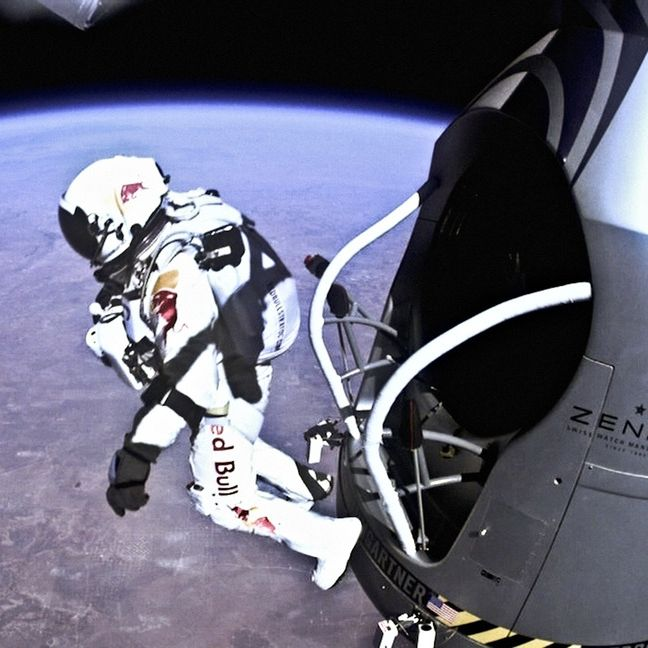
\includegraphics[width=\linewidth]{Red Bull Stratos}
    \caption{Side view}
  \end{subfigure}
  \hfill
  \begin{subfigure}{0.5\textwidth}
    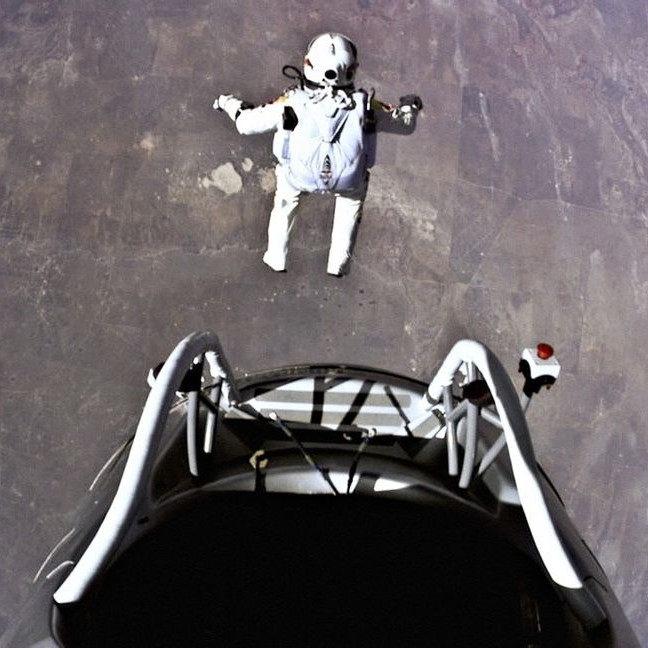
\includegraphics[width=\linewidth]{Felix Baumgartner}
    \caption{Top view}
  \end{subfigure}
  \caption{Felix Baumgartner space diving, October 14, 2012}
\end{figure}
%___________________________________________________________%
\subsection{Problem restatement}
We are going to analyze the challenges and dangers associated with the descent of a skydiver in a space suit with a parachute, propelled vertically by a rocket to an altitude potentially exceeding the Earth's atmosphere. Assuming that the total mass of the skydiver, space suit, and parachute is 190 $kg$, we will determine the maximum altitude from which an individual could safely return to the Earth's surface.
%___________________________________________________________%
\section{Assumptions and Notations}
\subsection{Assumptions}
We assume few things to avoid complexities in our estimation. Here are some of the key assumptions :
\begin{enumerate}
    \item[1.] We assume that the rocket, carrying the space diver, ascends vertically upward with no tangential velocity component.
    \item[2.] The diver jumps off the rocket with zero initial velocity relative to the ground.
    \item[3.] To simplify our model, we assume that the diver conducts the descent in such a way that no flat spinning is induced.
\end{enumerate}
If we need any further assumptions then we will state them throughout the text.
%___________________________________________________________%
\subsection{Notations}
\begin{table}[H]
\centering
\def\arraystretch{1.4}
\begin{tabular}{lp{4in}}
\hline
Symbols & Explanations \\ \hline
$F_g$ & Gravitational Force \\
$F_d$ & drag force \\
$F_{net}$ & Net Force \\
$G$ & Gravitational constant \\
$g$ & Gravitational acceleration at the sea level \\
$M$ & Mass of the Earth \\
$R$ & Radius of the Earth \\
$m$ & Mass of the space diver \\
$x$ & Altitude of the space diver from the sea level \\
$v$ & Velocity of the space diver \\
$v_T$ & Terminal velocity of the space diver \\
$a_{net}$ & Net acceleration on the space diver \\
$\rho$ & Density of the air \\
$C_d$ & Drag Coefficient \\ 
$A$ & Surface area\\
\hline
\end{tabular}
\end{table}
%___________________________________________________________%
\section{Challenges and Analysis}
There are many serious challenges and dangers associated with space diving. These challenges have to be acknowledged to ensure the safe descent of the diver, otherwise catastrophic events may occur. In this section we acknowledge some of these challenges and analyze their effects on the space diver.\\
%___________________________________________________________%
\textbf{(1) Hypoxia:} Hypoxia refers to the situation when the tissue of the body is depleted of enough oxygen which they need to maintain adequate homeostasis. At an extreme altitude required for space diving, the air density is so inadequate that the capsule or the rocket needs to provide oxygen to the space diver during the ascent via a liquified oxygen source and the space suit needs to provide 100 percent oxygen via a high-pressure gaseous oxygen cylinder during  descent. Minor hypoxia can cause impaired judgment and coordination, which can lead to unrecoverable flat spin. Without a properly functioning space suit the space diver may fall victim to hypoxia, which can eventually lead to death.
To prevent hypoxia we can take several steps as:

\textup{(i)} Using supplemental oxygen from takeoff until landing.

\textup{(ii)} Pre-breathing oxygen before takeoff.

\textup{(iii)} Ascending and descending slowly.\\
%___________________________________________________________%
\textbf{(2) Pressure for Skydivers:}
Skydivers are exposed to a variety of pressures during a skydive, including atmospheric pressure, air resistance, and the force of gravity. It is important to know how these pressures work and how they affect the body.

\textbf{Atmospheric Pressure:}
Atmospheric pressure is the force exerted by the weight of the air above us. It decreases with altitude.
Pressure on Earth varies with the altitude of the surface, so air pressure on mountains is usually lower than air pressure at sea level. Pressure varies smoothly from the Earth's surface to the top of the mesosphere. Although the pressure changes with the weather, NASA has averaged the conditions for all parts of the earth year-round. As altitude increases, atmospheric pressure decreases. One can calculate the atmospheric pressure at a given altitude. Temperature and humidity also affect the atmospheric pressure. Pressure is proportional to temperature and inversely proportional to humidity. And it is necessary to know both of these to compute an accurate figure. The below graph was developed for a temperature of 15 °C and a relative humidity of 0\%. At low altitudes above sea level, the pressure decreases by about 1.2 $kPa$ (12 $hPa$) for every 100 meters\citep{springerBarometricFormula} :
$$P=P_0e^{  \frac{mgH}{kT}  }$$
%___________________________________________________________%
\begin{figure}[H]
\centering
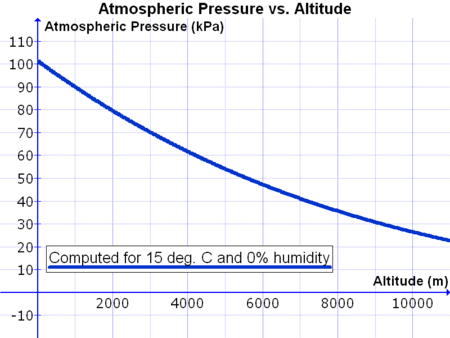
\includegraphics[width=0.6\linewidth]{baroform.png}
\caption*{\textbf{Figure:} Pressure variation with Altitude}
\end{figure}
%___________________________________________________________%
\textbf{Ebullism:} The boiling point of water decreases with altitude. This means that water in the body can boil at lower temperatures. This can cause ebullism, which is the formation of bubbles in the bloodstream and body tissues. Ebullism can also be fatal.

\textbf{Air Resistance :}
Air resistance is the force that opposes the motion of an object through the air. It increases with speed, so skydivers experience more air resistance as they freefall. Air resistance can cause a number of physiological effects, including

\textbf{Windblast:} This is the force of the wind blowing against the body. It can cause discomfort, dry eyes, and even difficulty breathing.
G-forces: G-forces are the forces that act on the body during acceleration or deceleration. Skydivers experience positive G-forces when exiting the aircraft and negative G-forces when deploying their parachutes.\\
%___________________________________________________________%
\textbf{(3) Difficulties due to extreme temperature :} The temperature of the atmosphere varies wildly as a function of altitude. A figure depicting these variation is shown below :
%___________________________________________________________%
\begin{figure}[H]
\centering
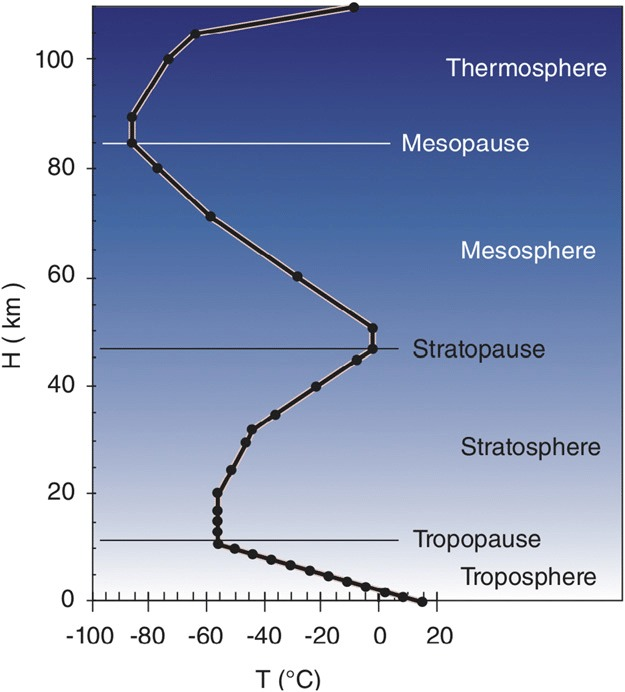
\includegraphics[width=0.6\linewidth]{temp.jpeg}
\caption*{\textbf{Figure:} Temperature variation with Altitude}
\end{figure}
%___________________________________________________________%
From the above figure we can see that the temperature gets as low as \SI{-90}{\degreeCelsius} at an altitude of 85 km which is extremely cold. Hence, the space suit that the diver wears must have the capability to keep the diver safe from this extreme cold. Otherwise the diver may face severe consequences\citep{baldwin2019progress}.\\ \\
%___________________________________________________________%
\textbf{(4) Flat Spin:} Flat spin is the term which refers to the rapid rotation of a space diver with respect to the axis which is perpendicular to the ground. This can occur due to asymmetric position of the diver or due to initial rotational motion while jumping. Many other factors are associated with this phenomenon. This rotation can be deadly for a space diver since due to this spin the pseudo centrifugal force on the blood of the space diver will cause blood pressure to rise on the head of the diver. This much blood pressure on the head can cause blindness, unconsciousness and even death.In case of low altitude sky diving this spin can be eliminated by certain maneuver of the body, because there is ample amount of air to provide drag force against the spin. However, in case of extreme diving altitude the effect of the spin is more severe, since at such an altitude the air density is so low that there will be no way to recover from this deadly spin.\\
We will approach to estimate the centrifugal force on the body and blood of the space diver with the following assumptions :

We assume the space diver as a cylindrical object with length 2r, where r = average half height of a human $\approx0.8 m$. We also assume the angular velocity of the space diver to be, $\omega = 4\pi$ $rads^{-1}$ (two revolutions per second). Now, the centrifugal acceleration will be, 
%___________________________________________________________%
\begin{align*}
    a_c &= \omega^2 r\\
        &= (4\pi \text{ }rads^{-1})^2 \times 0.8\\
        &= 126\text{ }ms^{-2}=12.9\text{ }g
\end{align*}
%___________________________________________________________%
At an extreme altitude this amount of centrifugal force is more than enough to make the diver unconscious which can eventually lead to death. Hence flat spin is an important parameter which needs consideration to evaluate the maximum altitude for safe descent.
%___________________________________________________________%
\begin{figure}[H]
\centering
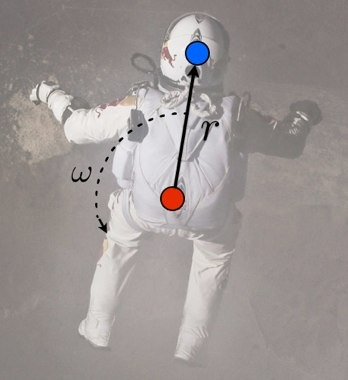
\includegraphics[width=0.6\linewidth]{flat-spin.jpeg}
\caption*{\textbf{Figure : }Flat Spin}
\end{figure}
%___________________________________________________________%
\section{Problem Analysis}
The problem here stands to estimate the maximum altitude for space diver's safe descent. By considering the assumptions stated earlier, we now approach to analyze the problem.\\
We know that while an object from rest undergoes free fall through the atmosphere, the object will experience two major forces :\\ the gravitational force and the drag force due to air friction.\\
%___________________________________________________________%
\textbf{Gravitational force ($F_g$):}
If the gravitational acceleration for an object at an altitude $x$ above the sea level is expressed with : $$g=\frac{GM}{(R+x)^2} $$
Then the gravitational force exerted the object by the Earth with mass m which is at an altitude of $x$ from the ground is expressed with :\\
$$F_g =\frac{GMm}{(R+x)^2}=mg$$ 
%___________________________________________________________%
\textbf{Drag force ($F_d$):}
drag force is mechanical force which is generated by the interaction and contact of a solid body with a fluid (liquid or gas). The expression for the drag force is :
$$F_d = \frac{1}{2} \rho v^2 C_d A $$

Hence, the net force on the falling object will be \citep{kincanon1990} :
%___________________________________________________________%
\begin{align*}
F_{net} &= F_g - F_d \\
\text{or, } m \frac{d^2x}{dt^2}&=mg-\frac{1}{2} \rho v^2 C_d A
\end{align*}
%___________________________________________________________%
\\Therefore,
%___________________________________________________________%
\begin{align}
\frac{d^2x}{dt^2}&=g-\frac{1}{2} \rho v^2 C_d \frac{A}{m} = a_{net} = g(x, v, t)
\end{align}
%___________________________________________________________%
and velocity, $v$ is the rate of change of the displacement, $x$ thus,
%___________________________________________________________%
\begin{align}
\frac{dx}{dt} &= v = f(x, v, t)  
\end{align}
%___________________________________________________________%
We can see from the expression of the drag force is proportional to the square of the velocity. So, when the object starts it's motion from zero velocity the drag force on the object is small compared to the downward gravitational force. Thus the object keeps accelerating and the velocity of the object keeps increasing. As a result of this increase in velocity, the drag force also increases over time. Eventually after some time, the object will reach such a velocity for which the drag force and the gravitational force cancel each other out. In this situation, the net force on the object is zero. Hence this critical velocity remains constant throughout the remaining fall. This critical velocity is called the terminal velocity of the object. The condition to achieve the terminal velocity is:
%___________________________________________________________%
\begin{align*}
F_{net}&=F_g - F_d=0 \\
&=mg-\frac{1}{2} \rho v_T^2 C_d A=0
\end{align*}
%___________________________________________________________%
Thus,
%___________________________________________________________%
\begin{align}
v_T=\sqrt{\frac{2mg}{\rho A C_d}}
\end{align}
%___________________________________________________________%
\subsection {Analyzing the motion of a skydiver for :}
\subsubsection {Uniform Density}
At first we consider a simplified hypothetical case where the air density remains constant throughout the fall, i.e the air density is independent of altitude or any other parameter. Here we assume that the space diver is initially jumping from an altitude of 10 $km$ with zero initial velocity. So, at $t=\text{0 }s, x=\text{10000 }m, v=\text{0 } ms^{-1}$

Now we solve the differential equations (1) and (2) numerically to get the altitude $(x)$, velocity $(v)$ and net acceleration $(a_{net})$ as a function of time $(t)$. To evaluate the solution, we consider the frontal surface area of an adult human $A = \text{0.95 }m^2$ and the drag coefficient for an adult human body in belly-down position $C_d = 0.5$. We assume the air density at sea level to be, $\rho_0=\text{1.225 }kgm^{-3}$

The solutions are below:
%___________________________________________________________%
\begin{figure}[H]
\centering
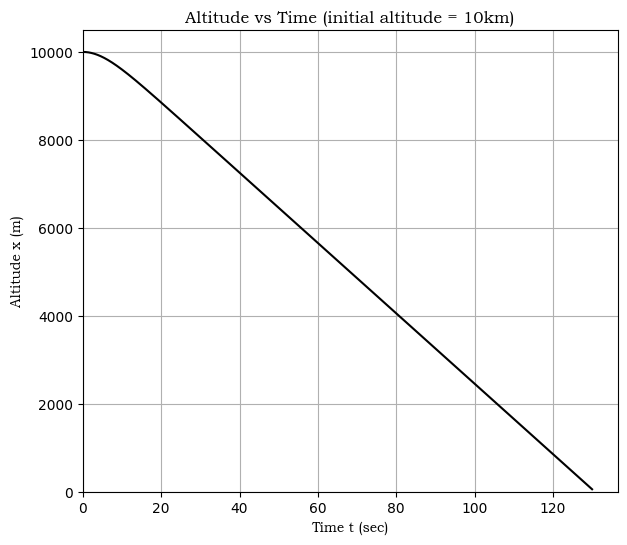
\includegraphics[width=0.5\linewidth]{10-1}
\caption{\label{10-1}Altitude vs Time}
\end{figure}
%___________________________________________________________%
\begin{figure}[ht]
  \begin{subfigure}{0.5\textwidth}
    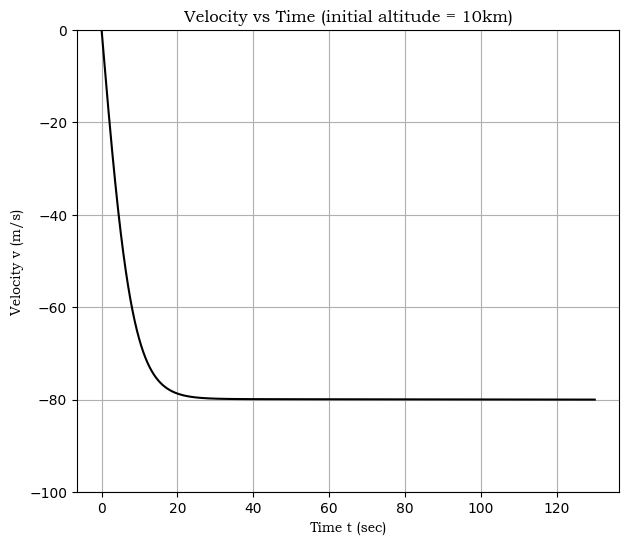
\includegraphics[width=\linewidth]{10-2}
    \caption{velocity vs time}
  \end{subfigure}
  \hfill
  \begin{subfigure}{0.5\textwidth}
    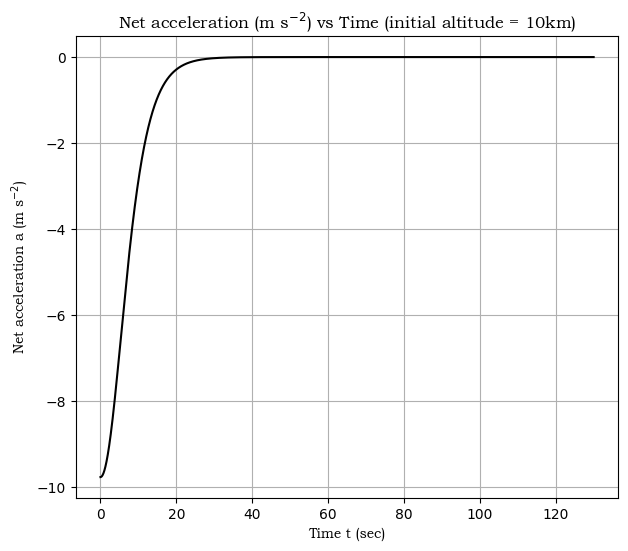
\includegraphics[width=\linewidth]{10-3}
    \caption{net acceleration vs t}
  \end{subfigure}
  \caption{v vs t and $a_{net}$ vs t for initial altitude = 10 $km$}
\end{figure}
%___________________________________________________________%
We can see from Figure 4:(a) that after 20 $s$ time the velocity becomes almost constant. This is the terminal velocity for the space diver.

From Figure 4:(b) we can see that initially $a \approx-\text{9.8 }ms^{-2}$ which decreases in magnitude with time to reduce to zero.
%___________________________________________________________%
\subsubsection {Variable Density}
Earlier, we considered a hypothetical scenario where the air density $(\rho)$ was independent of all parameters. However, in reality this is not the case since the air density $(\rho)$ depends on altitude $(x)$ and many other parameters. For simplicity, in this section we will consider the variation of $(\rho)$ with altitude $(x)$ only.  The density varies with altitude according to the relation:
$$\rho = \rho_0  e^{\frac{-x}{H}} $$ where,\\
$\rho(x)$ = air density at an altitude $x$ ,\\
$\rho_0$ = air density at sea level = 1.225 $kg/m^3$ ,\\
$H$ = scale height = 7000 $m$\\
The relation stated above is called the barometric formula (for air density)\citep{wiki-barometric-formula}. From this relation we can see that air density decreases exponentially with increasing altitude.
%___________________________________________________________%
\begin{figure}[H]
\centering
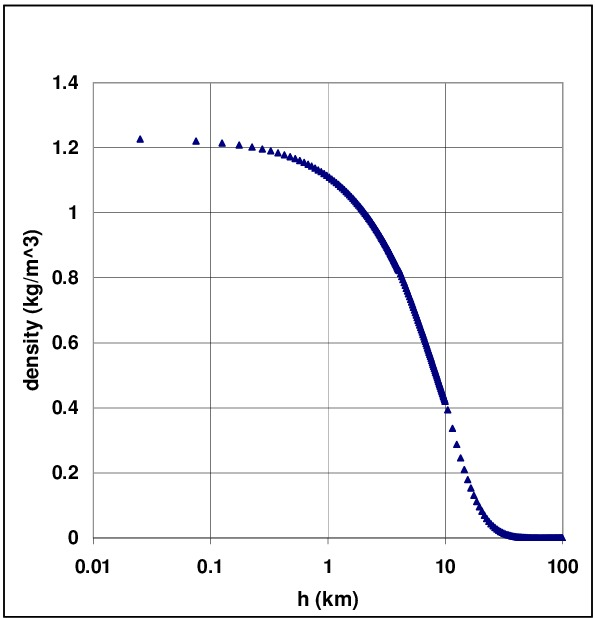
\includegraphics[width=0.5\linewidth]{rho-variation.jpeg}
\caption{\label{fig:rho-variation}Density of air as a function of the vertical altitude above the level. \citep{anchordoqui2000air}}
\end{figure}
%___________________________________________________________%
Hence, if the space diver dives from a very high altitude, the drag force on them will be very low, similar to the case as if there is no resistance due to air. As a result, the space diver's velocity can become much greater than the case where we assumed uniform air density. However, during this descent, when the diver reaches an altitude lower than approximately 15-20 $km$ with very high speed, the drag force starts to play a significant role. Due to the high speed, the drag force eventually overcomes gravity and the net acceleration acts upward. The higher the initial diving altitude, the greater the net acceleration can become. At high altitude under critical conditions, a space diver in a pressurized suit can withstand around 5g for a few seconds. \citep{park2015unpredictability}.

If the diver dives from such an altitude that the maximum g-force on the diver exceeds this value then we can conclude that this value of altitude is too high for a safe descent of the diver.
Hence, the goal is here to estimate such an altitude for which the maximum g-force will be at maximum around 5g.
We will consider two initial altitudes separately, one is 40 $km$, which is about the same altitude as the world record space dive performed by Alan Eustace  and the other is 130 $km$ which is the altitude we are seeking for, for which the maximum upward g-force is roughly 5g.
In the case of diving altitude of 40 $km$, the numerical solutions for the velocity and the g-force as a function of time is given below -\\
%___________________________________________________________%
\begin{figure}[ht]
  \begin{subfigure}{0.5\textwidth}
    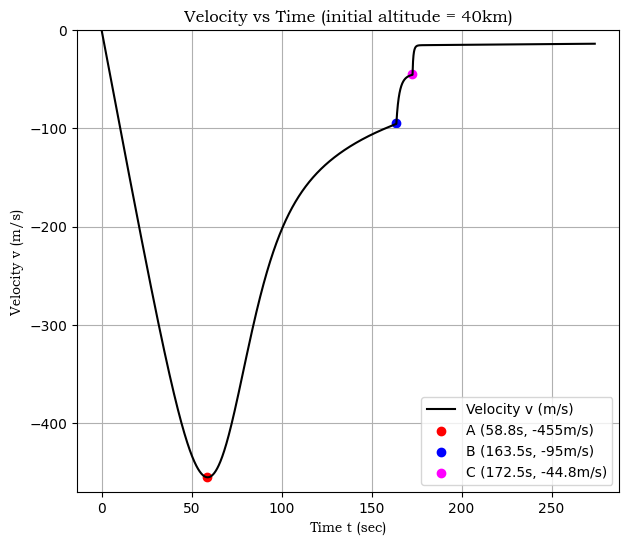
\includegraphics[width=\linewidth]{40-2}
    \caption{v vs t}
  \end{subfigure}
  \hfill
  \begin{subfigure}{0.5\textwidth}
    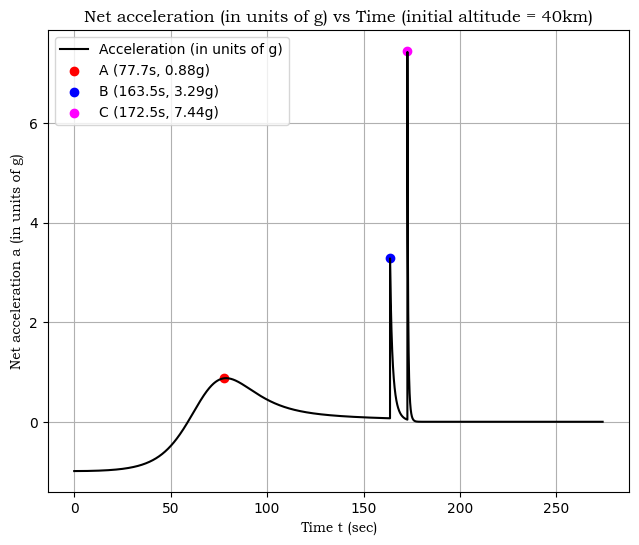
\includegraphics[width=\linewidth]{40-3}
    \caption{g vs t}
  \end{subfigure}
  \caption{v vs t and g vs t for initial altitude = 40 $km$}
\end{figure}\\
%___________________________________________________________%
From the data file of the numerical solution and the above graph we can see that the maximum velocity reached in this case is around 455 $ms^{-1}$ which is around mach 1.3. The maximum g-force in this case is around 0.9g. Despite being very challenging and dangerous, neither of these were too extreme to be a limiting factor of such a space jump. Hence such a descent was achievable safely. In the case of 130 $km$, the numerical solutions for the velocity and the g-force as a function of time is given below :
%___________________________________________________________%
\newpage
\begin{figure}[ht]
  \begin{subfigure}{0.5\textwidth}
    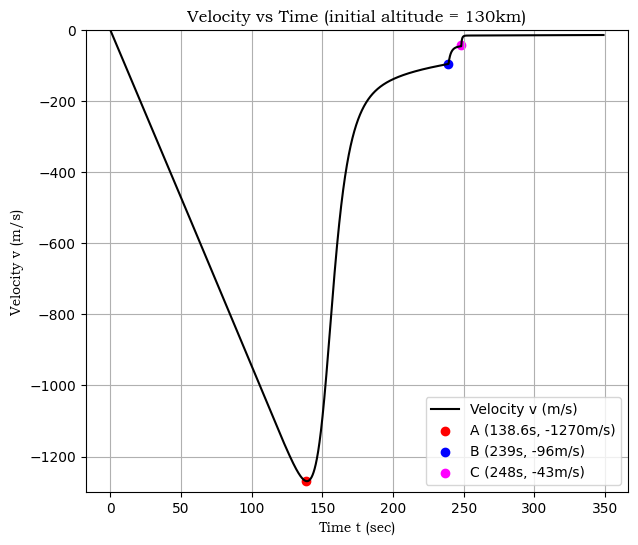
\includegraphics[width=\linewidth]{130-2}
    \caption{v vs t}
  \end{subfigure}
  \hfill
  \begin{subfigure}{0.5\textwidth}
    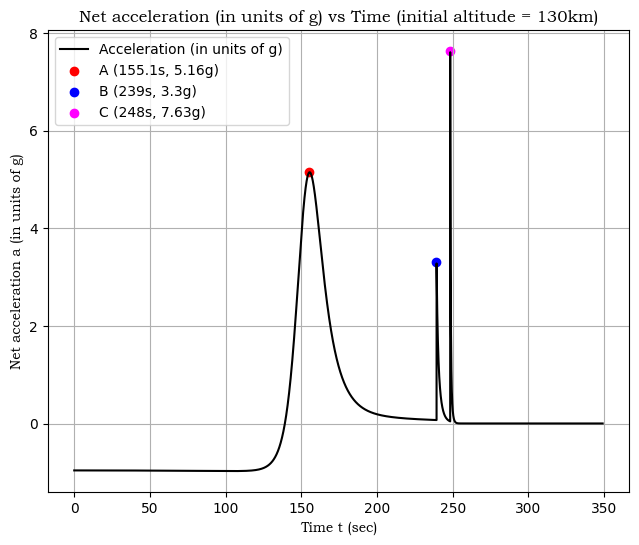
\includegraphics[width=\linewidth]{130-3}
    \caption{g vs t}
  \end{subfigure}
  \caption{v vs t and $a_{net}$ vs t for initial altitude = 130 $km$}
\end{figure}
%___________________________________________________________%
Similarly as before, we can see that the maximum velocity in this case 1270 $ms^{-1} $$\approx3.7$ mach. The maximum g-force in this case is around $5.16g$, which is the threshold g-force for safe descent. From the graph we can see that the duration during which the diver experiences more than 4g while entering the thick atmosphere is approximately 10 seconds, which is considerable. Hence, if we do not consider the limitations associated with the hypersonic speed achieved during free fall at extreme high altitude then 130 $km$ will be the threshold altitude for safe descent of the sky diver.

The points B and C in the velocity vs time graphs represent the deployment of the drogue parachute and the main parachute respectively. We assumed the deployment of the drogue parachute at an altitude of 2000 $m$ and the main parachute at 1500 $m$.\\ The parameters used for the drogue parachute are : $$A = \text{2 }m^2, C_d = 0.95$$ and for the main parachute are : $$A =\text{9 }m^2, C_d = 1.75$$
which are the standard values for drogue and main parachute \citep{nasa-rocket-recovery}.

We can see that at point B the velocity decreased to approach the terminal velocity with a drogue parachute and again at point C the velocity decreases again to approach the terminal velocity with the main parachute which is around 10 $ms^{-1}$, which is safe for human landing.

In case of net acceleration (in g) vs time graphs the two spikes at point B and C indicate the sudden upward acceleration due to the drogue parachute and the main parachute respectively. Though our model suggests high g-force (around $3.3g$ for drogue parachute and $7.6g$ for the main parachute in both case) for very short duration of time (fraction of a second), in actual case the g-force due to parachute deployment does not reach such high value since the deployment does not happen instantaneously, instead it takes few time.
%___________________________________________________________%
\subsection{Consideration of the top speed during descent}
In the previous section we did not consider the effect of the top speed of the space diver on their safety. However, this top speed can be a major factor limiting the maximum altitude achievable for safe descent. In the previous section we saw that the top speed for descent from 40 $km$ was around mach 1.3 which was within the limit of modern space suit’s capability. But if we are to dive from a more extreme altitude than 40 $km$ then our top speed will be much greater than mach 1.3. In this scenario, the top speed may exceed the withstand capability of the modern space suit available at present. In this section we will hypothetically assume a few top speeds which can withstand by space suits and approach to find out the maximum altitude corresponding to those top speeds.\\ \\
\textbf{Top speed of mach 2 :} By trying with several diving altitude we found out that in case of $x_0=\text{60 }km$, our top speed is around 680 $ms^{-1}$  $\approx$ mach 2. The following figure shows the velocity profile of such a descent :
%___________________________________________________________%
\begin{figure}[H]
\centering
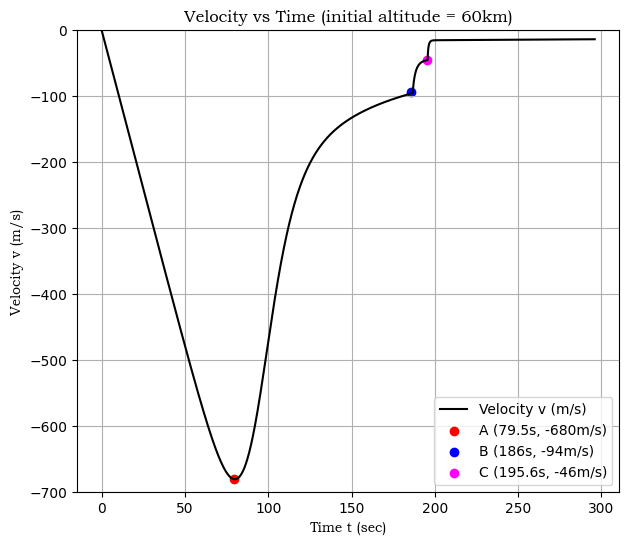
\includegraphics[width=0.7\linewidth]{figures/60-2}
\caption{\label{fig:615A/60-2}Velocity v ($ms^{-1}$) vs Time t (s)}
\end{figure}
%___________________________________________________________%
Similarly we found out that for top speed of mach 2.5, the initial altitude is around 80 $km$ and for top speed of mach 3, the initial altitude is around 100 $km$.
Hence, to exceed the initial altitude of 100 $km$ which is defined as the Karman line we will need such a suit which can protect the space diver from various life threatening effects of falling at supersonic speed of mach 3. Such a suit will be much heavier than 190 $kg$. Hence the top speed will be a limiting factor for the top altitude for safe descent. The result of this section can be summarized in a table as : 
%___________________________________________________________%
\begin{table}[H]
\centering
\caption*{}
\def\arraystretch{1.4}
\begin{tabular}{|l|p{2.2in}|}
\hline
\centering Top Speed & \centering\arraybackslash Corresponding altitude \\ \hline
\centering mach 2 & \centering\arraybackslash 60 $km$ \\ \hline
\centering mach 2.5 & \centering\arraybackslash 80 $km$ \\ \hline
\centering mach 3 & \centering\arraybackslash 100 $km$ \\ \hline
\end{tabular}
\end{table}
%___________________________________________________________%
\section{Evaluation}
\subsection{Evaluation of the Result}
According to our model, the speed of the space diver during fall from an altitude of 40 $km$ is 455 $ms^{-1}$. In the real life case Felix Baumgartner, who jumped from an altitude of 39 $km$ achieved a top speed of 377 $ms^{-1}$. This deviation of top speed is due to the mass difference in our problem and the real case. In our problem we assumed a space diver along with their diving gear to have a mass of 190 $kg$. But in the case of Felix Baumgartner, the total mass was around 110 $kg$. Due to the higher mass of the space diver stated in the problem than the real world event, we got faster speed.

We conclude that our estimates for the highest altitude for safe descent are consistent with real-world results.
%___________________________________________________________%
\subsection{Evaluation of Model}
\subsubsection{Strengths}
\begin{enumerate}
    \item[1.]Our model is very simple and easy to solve and analyze using python codes and plots.
    \item[2.] It gave us an estimate of the maximum altitude which can be considered safe for a space diver descent in a very short duration of time.
    \item[3.] Our model is based on very basic principles of physics which will make this model understandable to a wider range of audience.
    \item[4.] Numerous figures and graph plots are provided to make understanding the paper easier.
    \item[5.] The terminal velocities in various cases of our analysis match with the real life data.
    \item[6.] Our results for the dive from 40 km agrees pretty well with the real life results, which were obtained from the space dives of Felix Baumgartner and Alan Eustace.
\end{enumerate}
%___________________________________________________________%
\subsubsection{Weaknesses}
\begin{enumerate}
    \item[1.]We are not considering the amount of oxygen which is available during the descent. Since the suit must be capable of serving 100\% oxygen during free fall at extreme altitude, hence the amount of oxygen available can be a limiting factor.
    \item[2.] Even though we showed that flat spin has a monumental effect on the safety and the maximum altitude of the dive, we did not consider it in our analysis in order to avoid complexity.
    \item[3.] We did not analyze the heating of the space suit during the descent which can be an important factor in estimating the maximum diving altitude.
    \item[4.] The momentary drag during parachute deployment was large, since we wrote our codes in such a way which is equivalent to deployment of parachute in no time. Since in the real scenario, parachute deployment requires some time, hence the drag force is not as large as predicted by our model during parachute deployment.
    \item[5.] We considered the initial velocity of the diver to be zero to avoid complexity, but this condition will be very hard to achieve in case of ascent via rocket.
    \item[6.] We considered the air density to be solely a function of altitude. However, in reality the air density depends on many other parameters, such as temperature, air humidity, compositions of gas etc.
    
\end{enumerate}
%___________________________________________________________%
\section{Conclusion}
If we do not consider the effect of supersonic speed, flat spin on the space suit and the space diver’s safety and only account the effect of g-force on the space diver due to the thickening atmosphere then the highest altitude from which a safe descent may be achieved is found out to be around 130 $km$.

If we also take into account the effect of supersonic speed on the space suit and the space diver’s safety then various top speed sets various maximum altitude. Those which are found in this paper are approximately 60 $km$, 80 $km$ and 100 $km$ for mach 2, mach 2.5 and mach 3 respectively. Hence, if a diver wants to dive from an altitude of more than 100 $km$ (which is the Karman line) then we must ensure that our space suit is capable of withstanding an speed of more than mach 3 while keeping the diver safe.

% References------------------------------------------------
% Add the bibliography section with numbered references
\addcontentsline{toc}{section}{References}
\bibliographystyle{unsrtnat}  % Specify the bibliography style (unsrtnat for numbered references)
\bibliography{615A-references}
\newpage
%___________________________________________________________%
\section*{Appendix}
\addcontentsline{toc}{section}{Appendix}
Python Codes:
%___________________________________________________________%
\begin{figure}[H]
\centering
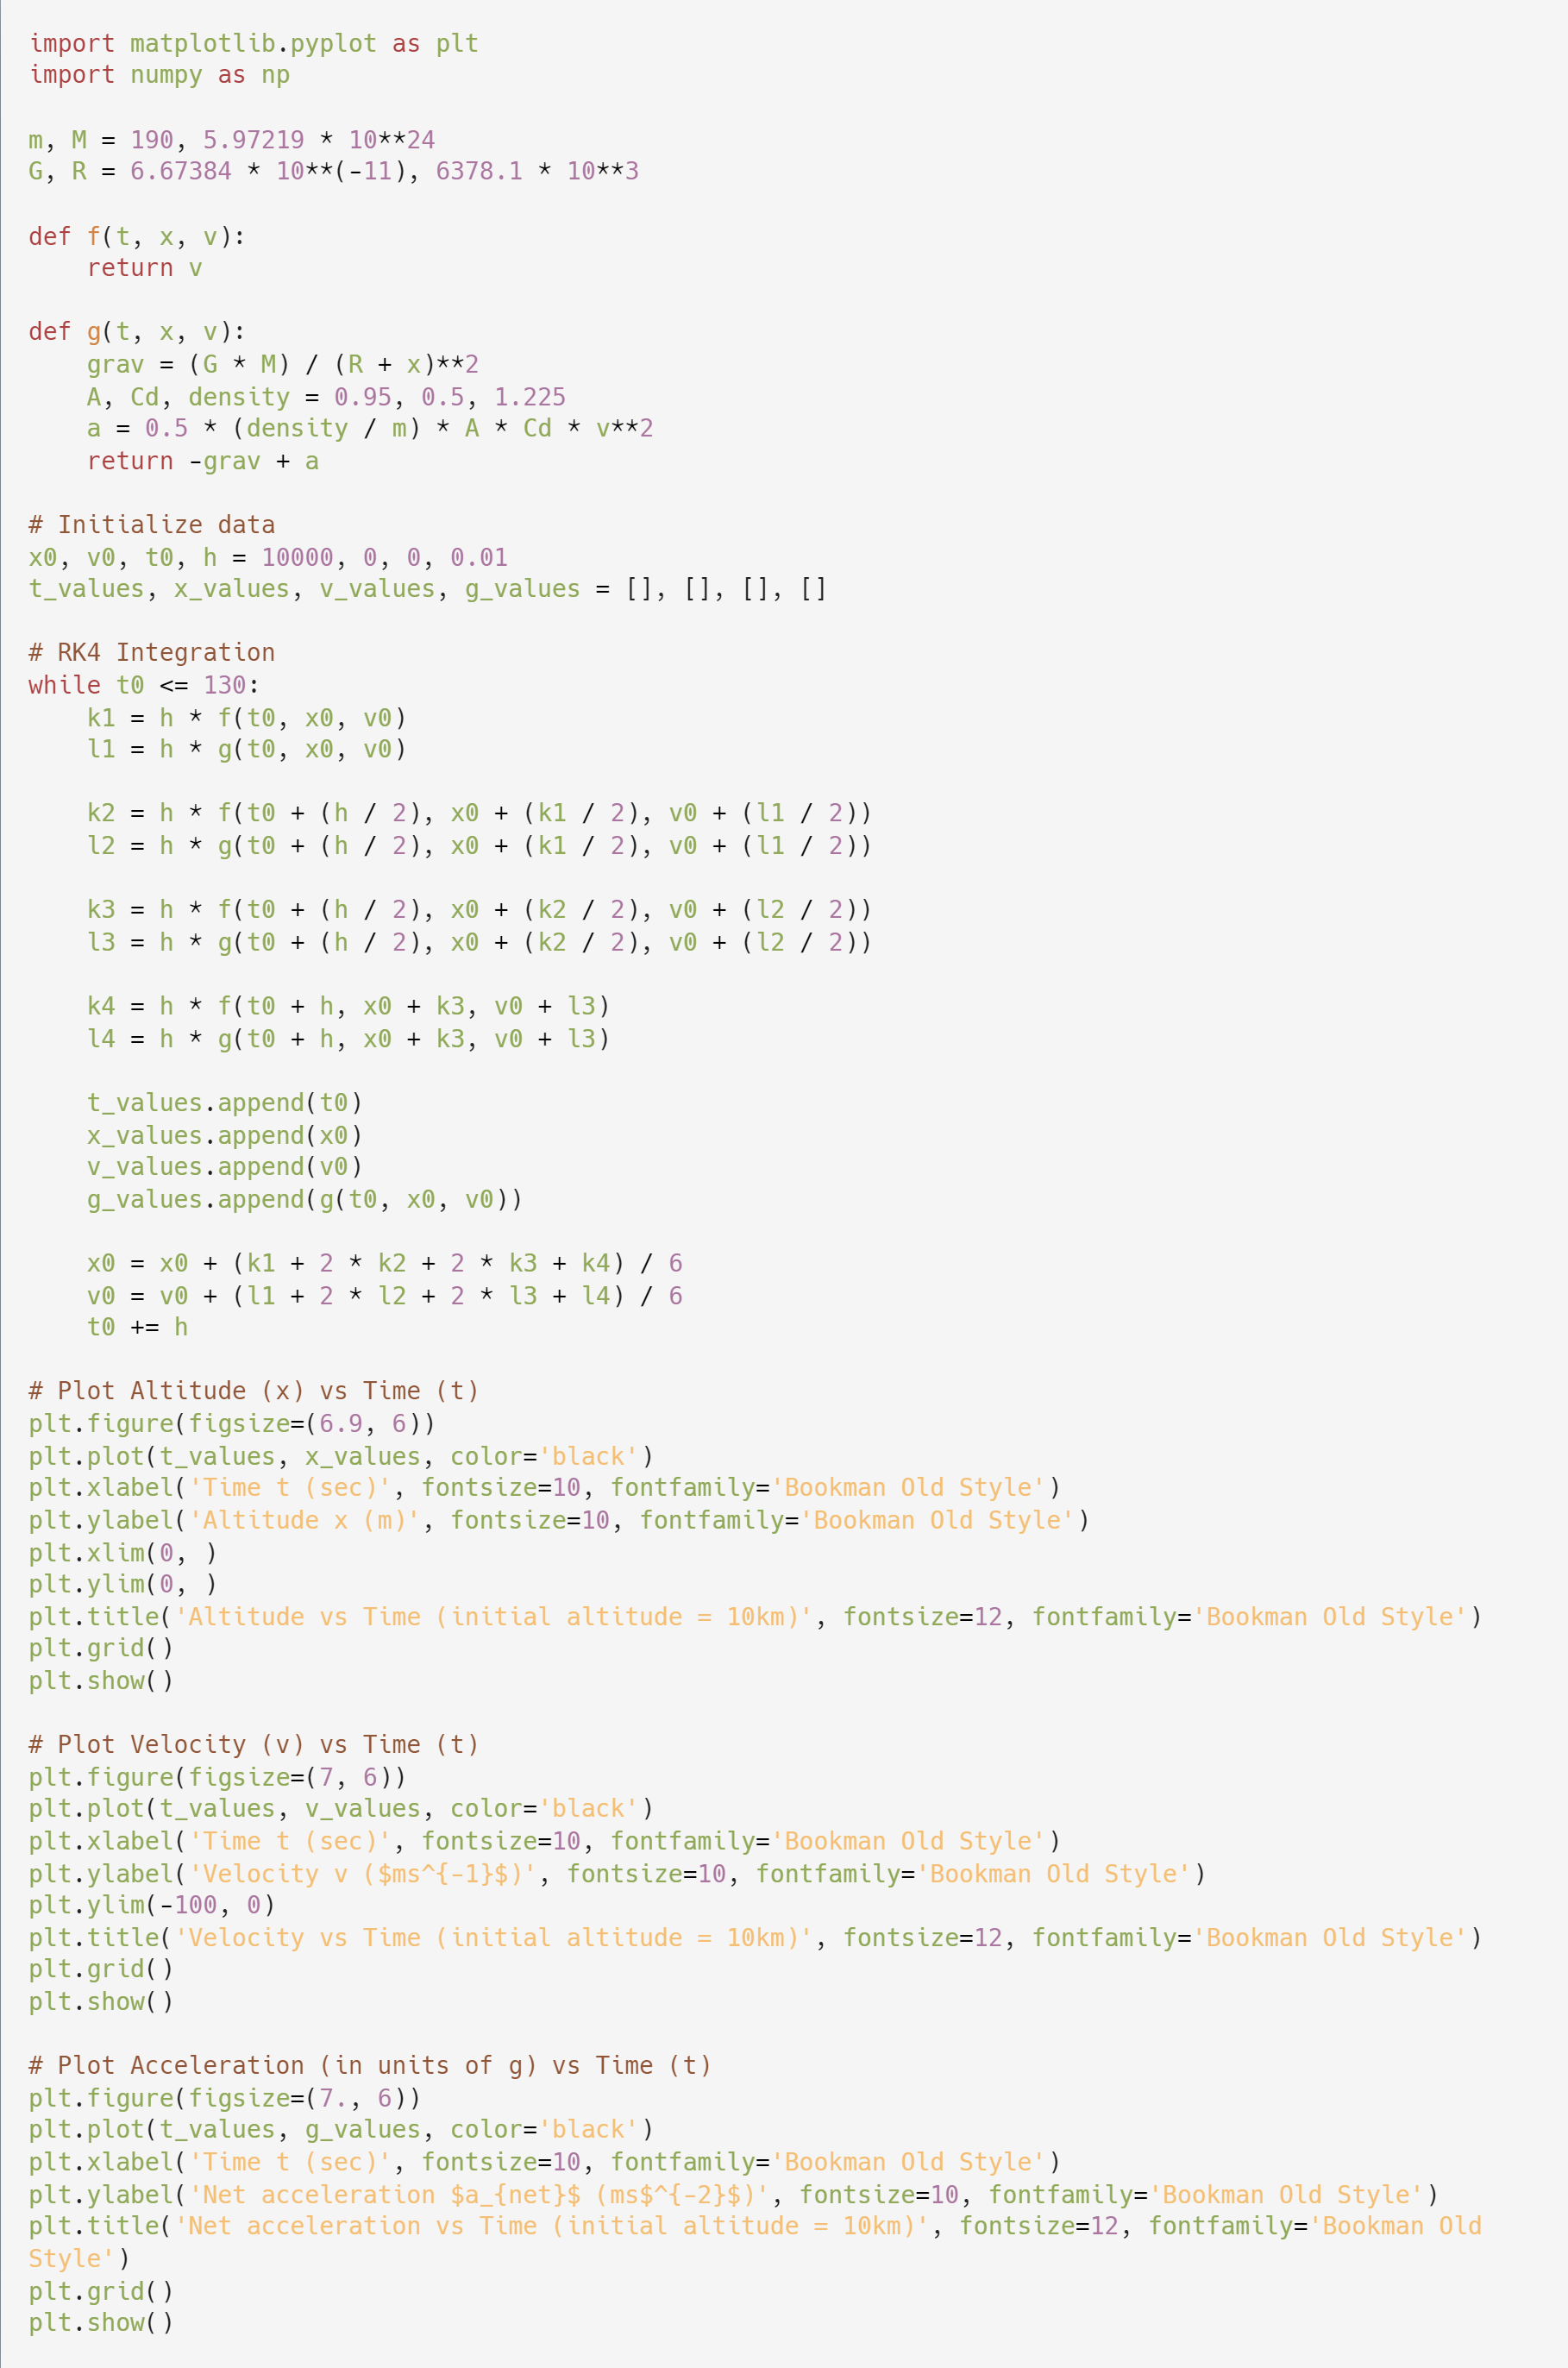
\includegraphics[width=0.77\linewidth]{1.png}
\caption*{}
\end{figure}
%___________________________________________________________%
\begin{figure}[H]
\centering
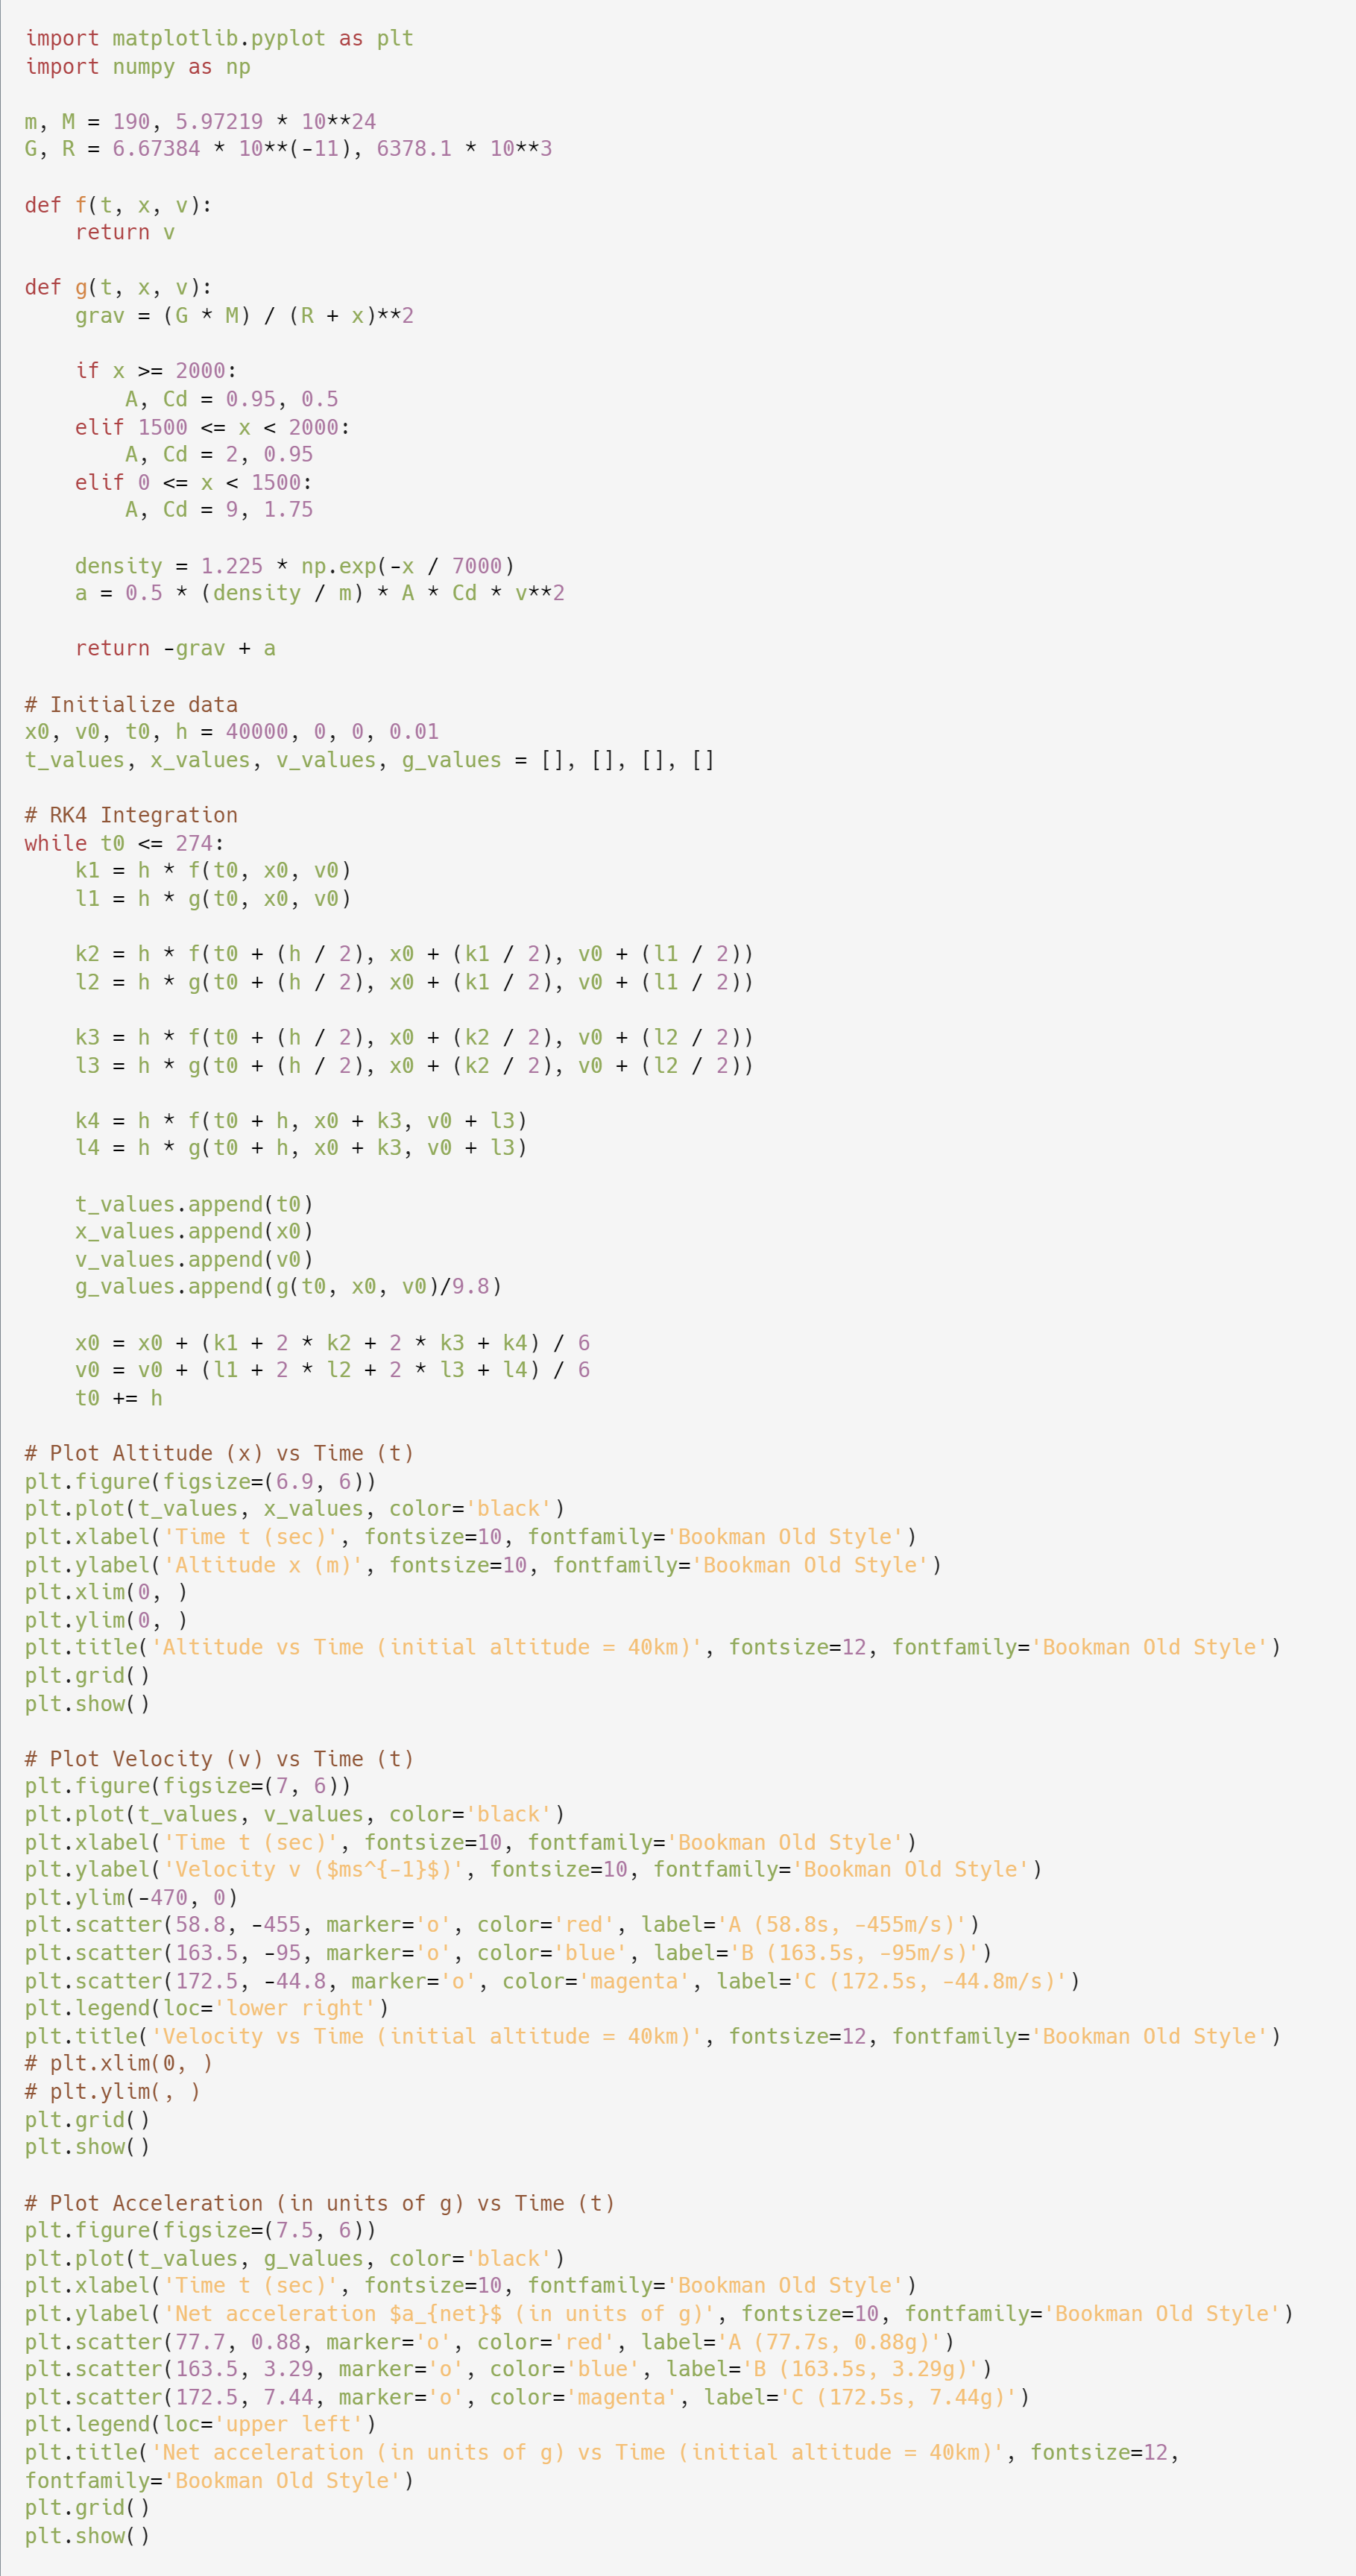
\includegraphics[width=0.87\linewidth]{2.png}
\caption*{}
\end{figure}
%___________________________________________________________%
\begin{figure}[H]
\centering
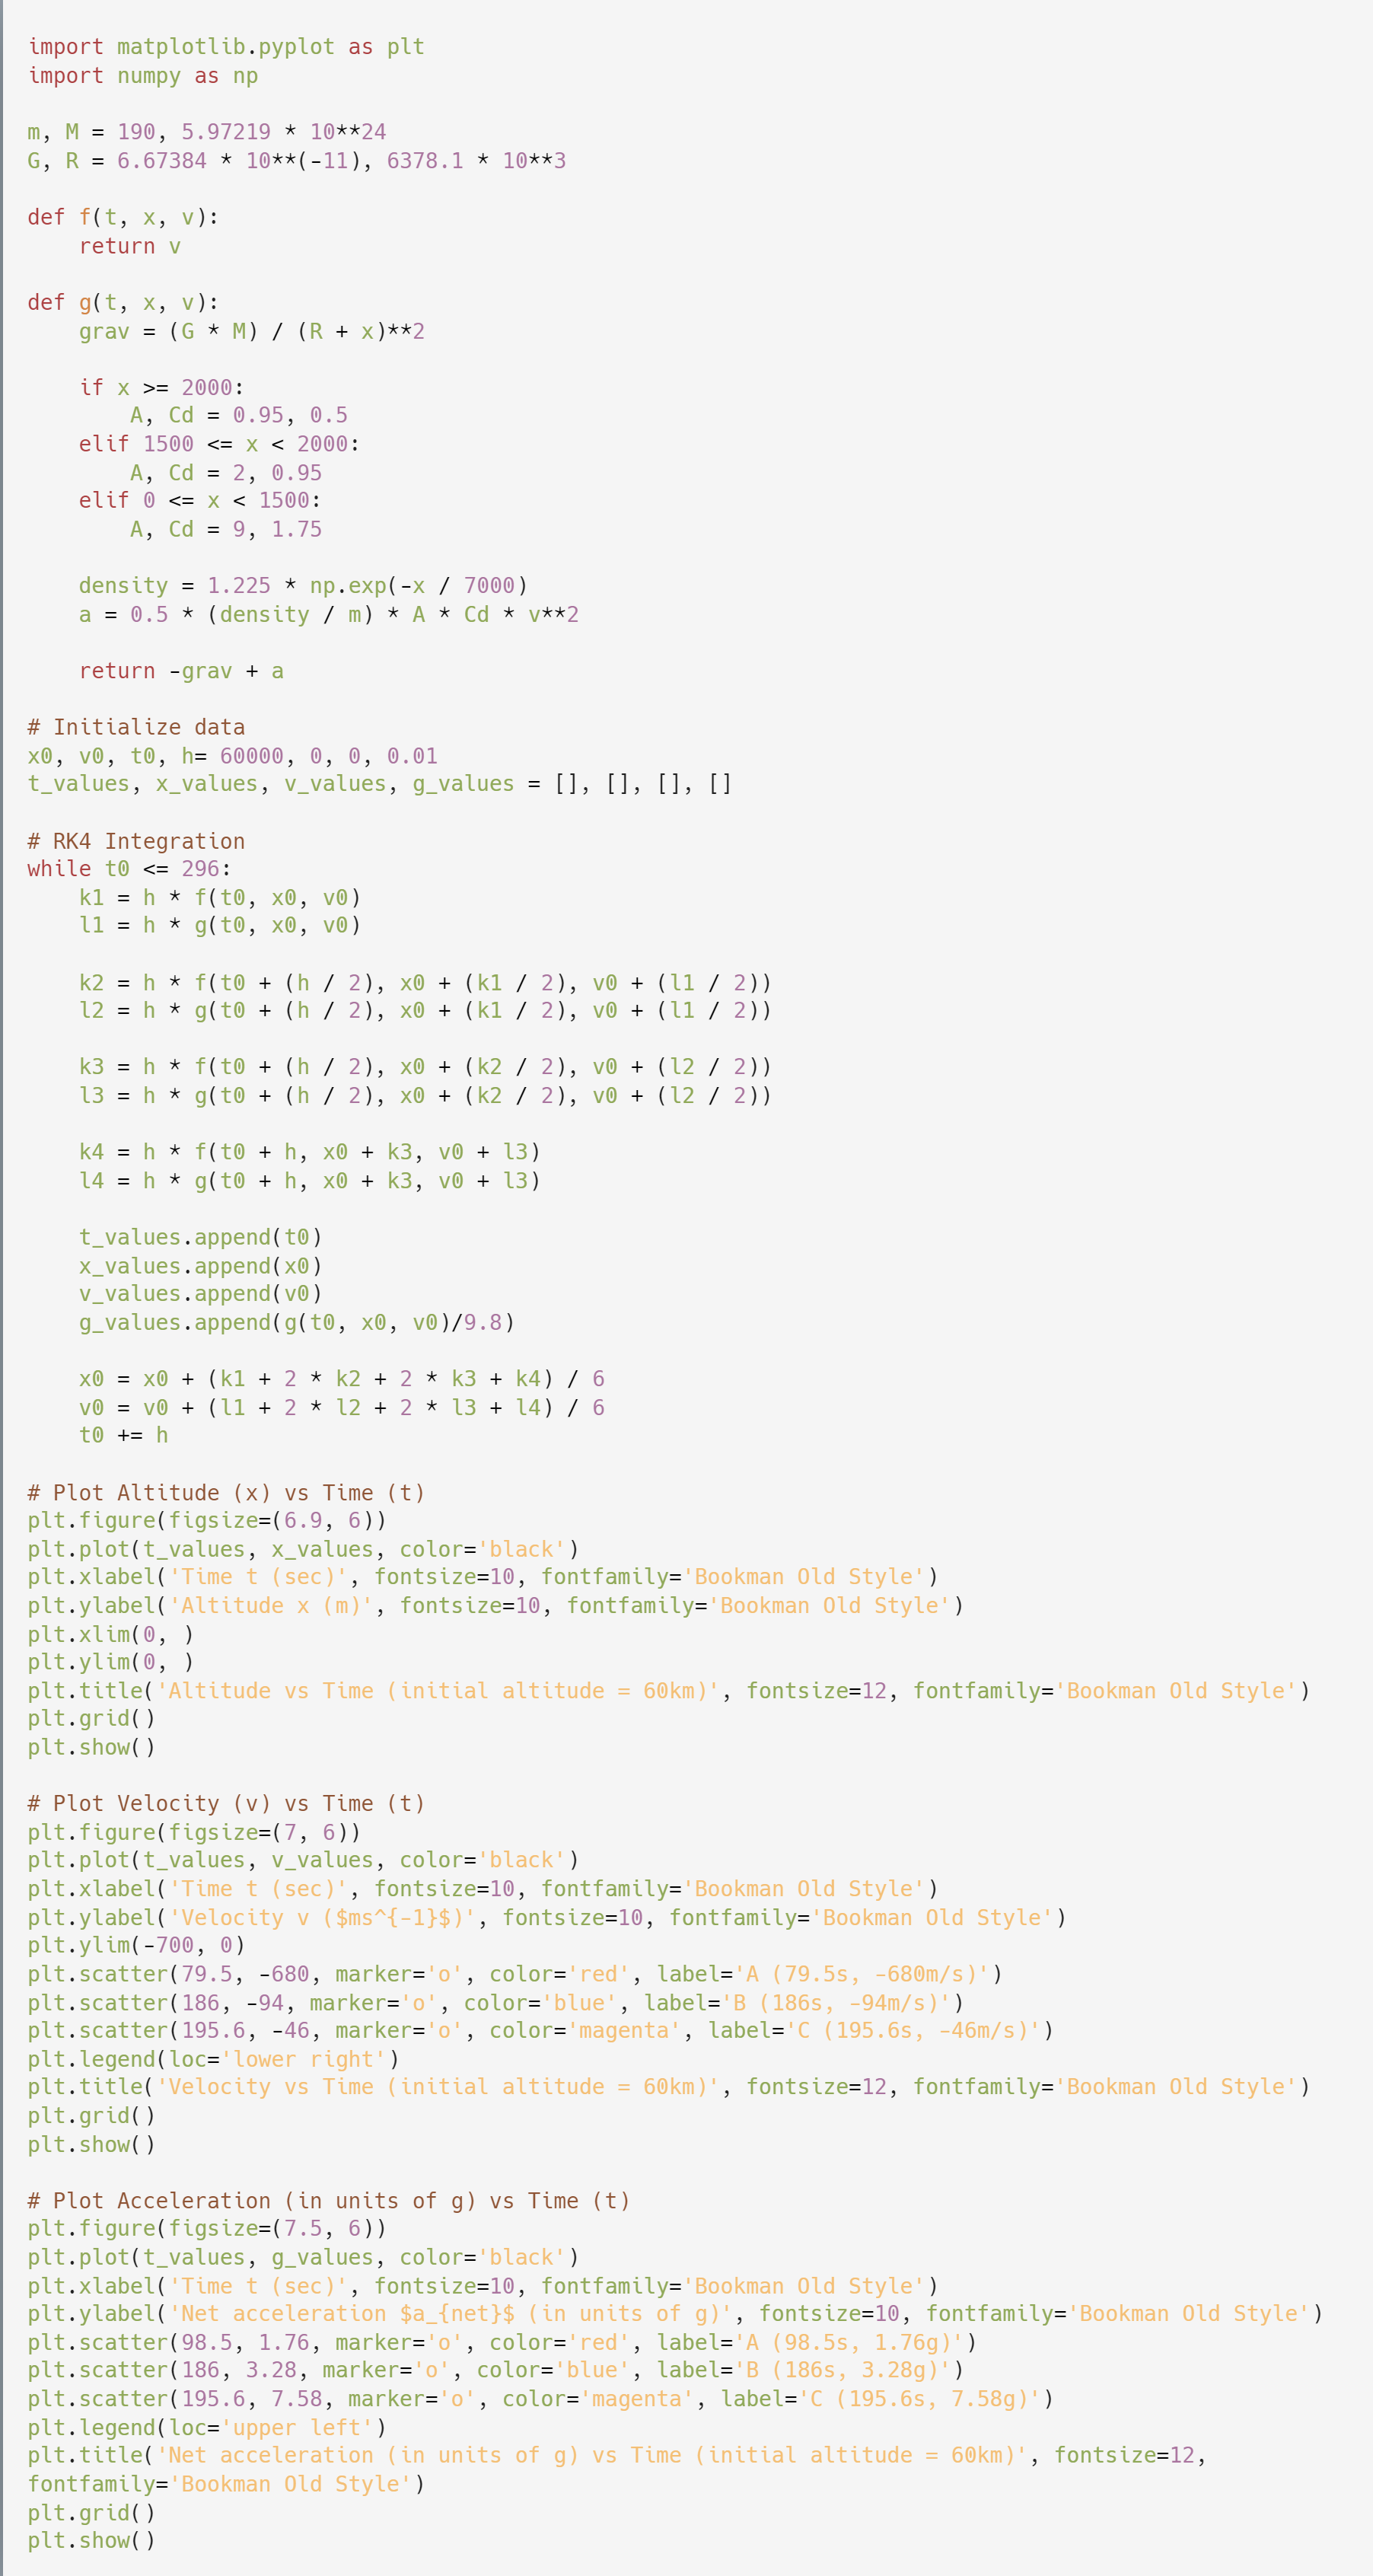
\includegraphics[width=0.87\linewidth]{3.png}
\caption*{}
\end{figure}
%___________________________________________________________%
\begin{figure}[H]
\centering
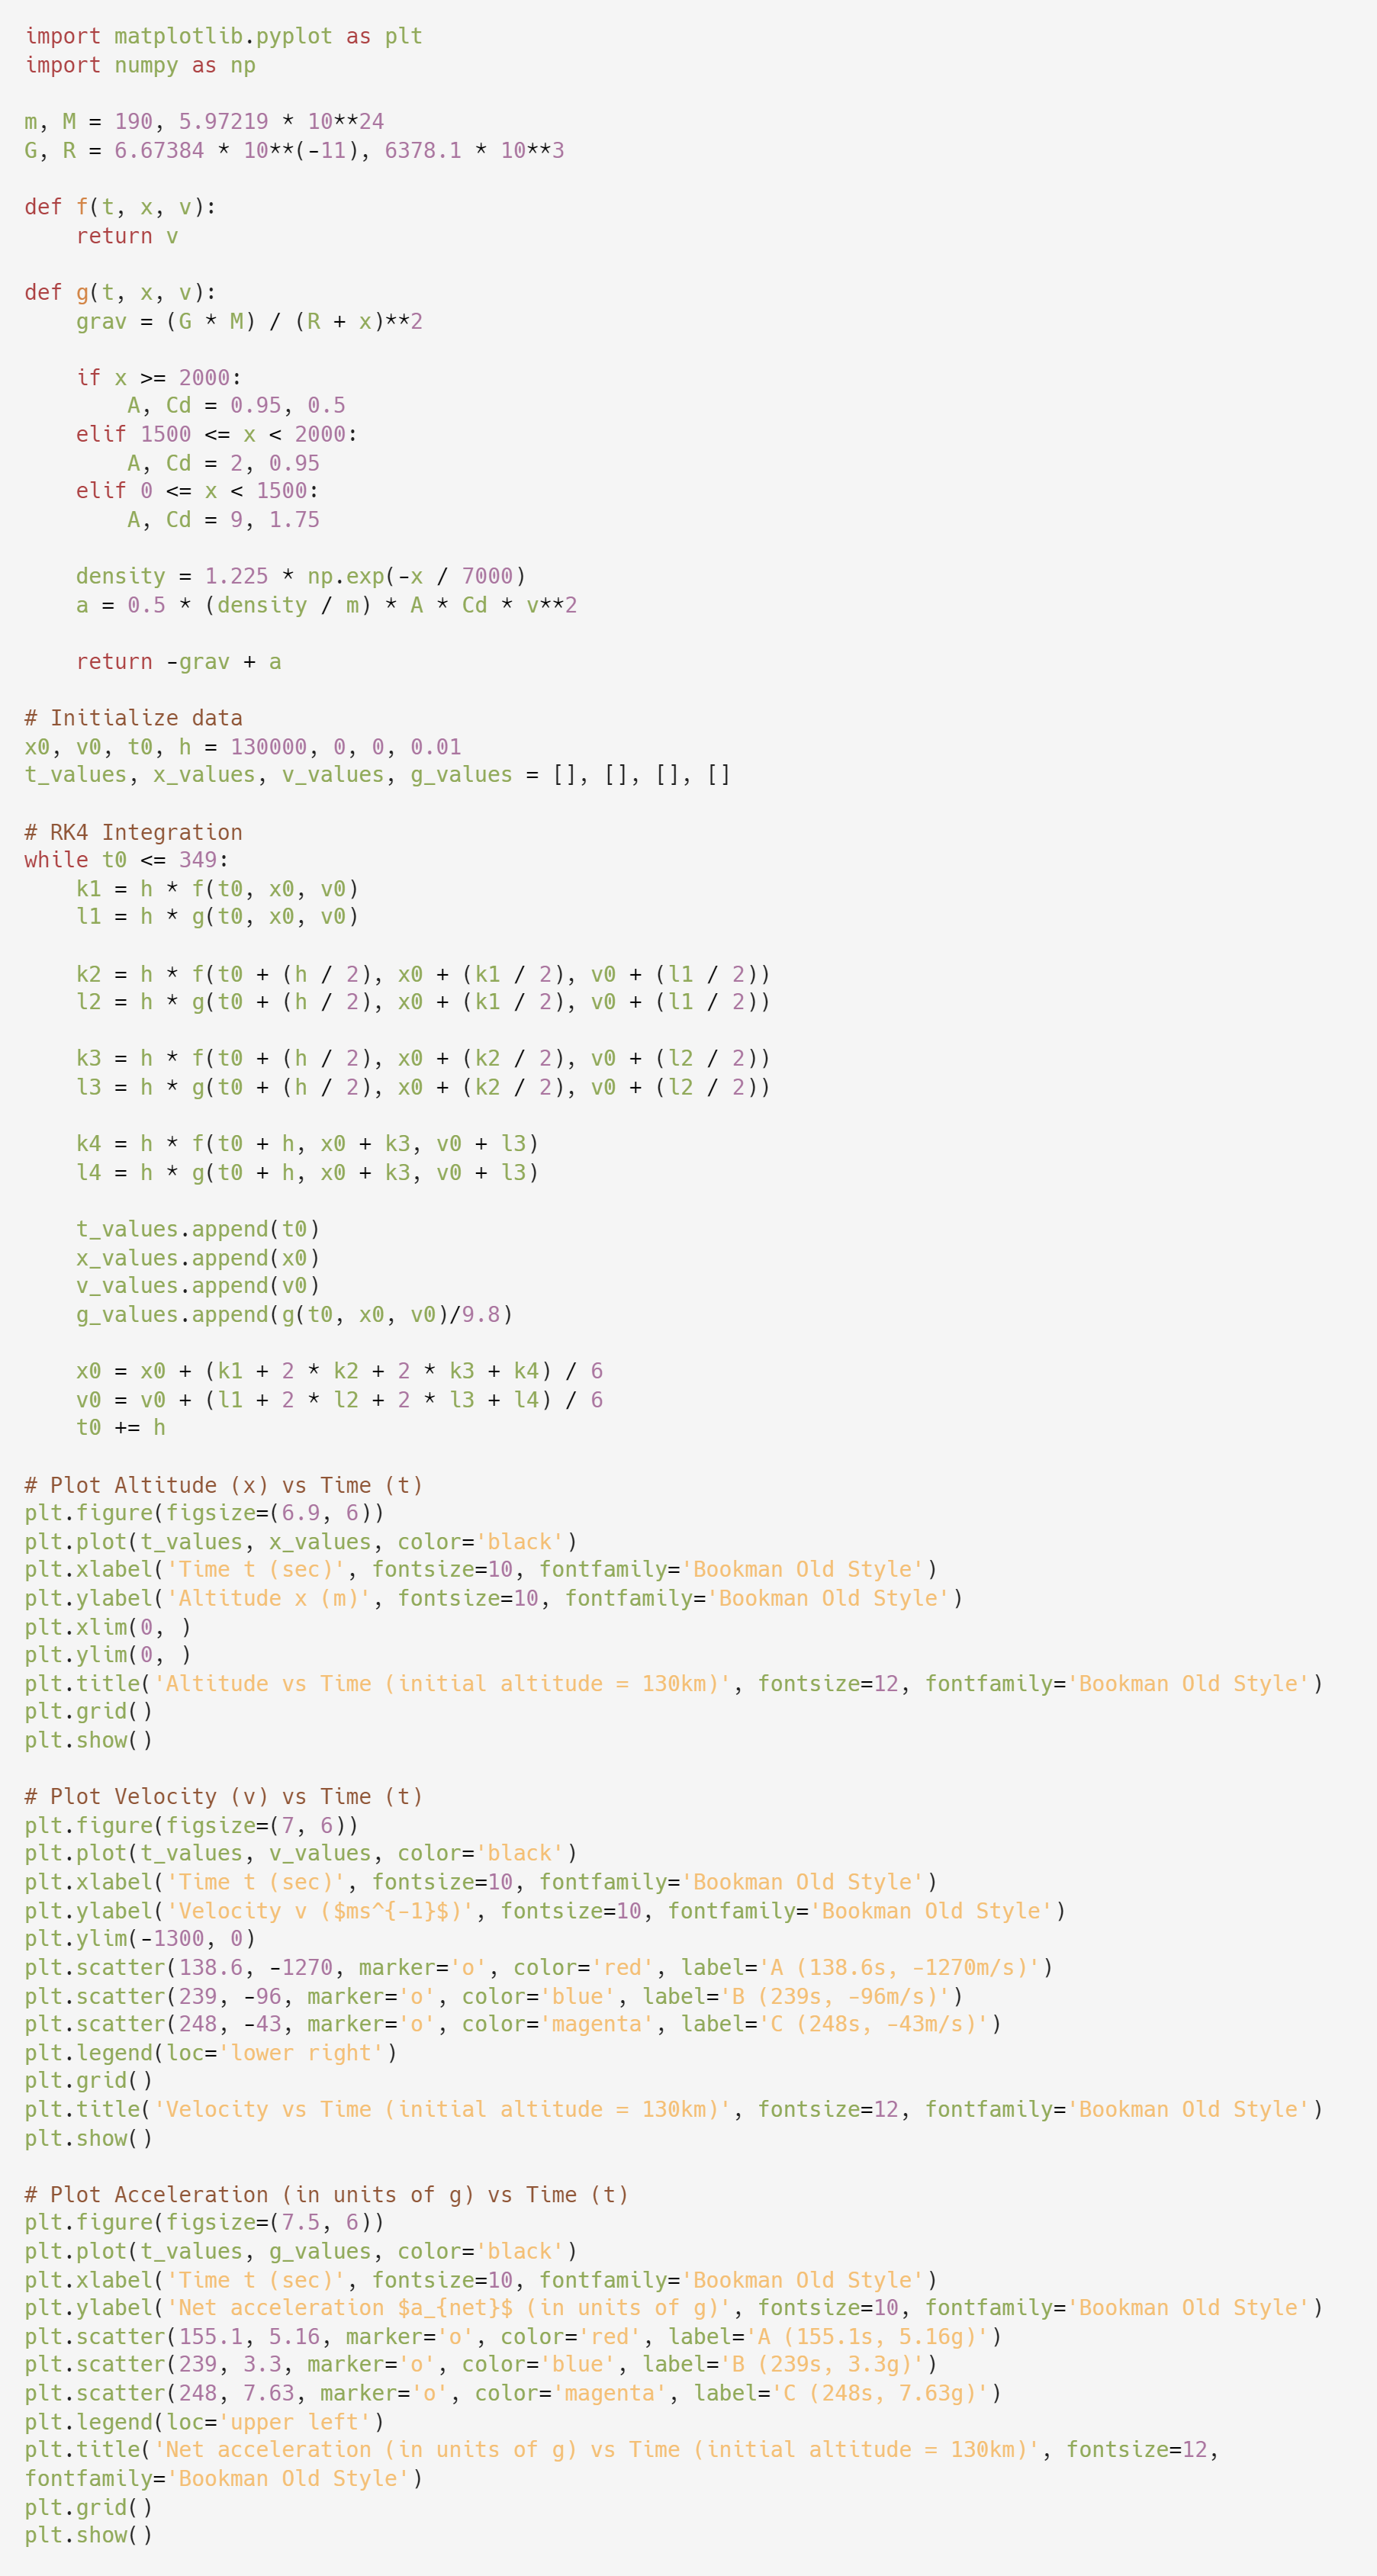
\includegraphics[width=0.87\linewidth]{4.png}
\caption*{}
\end{figure}
%___________________________________________________________%

\end{document}
